\documentclass[landscape, a0paper, debug]{baposter}

\usepackage{graphicx}
\usepackage{epstopdf}
\usepackage{multirow}
\usepackage{tikz}

\begin{document}

\definecolor{silver}{cmyk}{0,0,0,0.3}
\definecolor{yellow}{cmyk}{0,0,0.9,0.0}
\definecolor{reddishyellow}{cmyk}{0,0.22,1.0,0.0}
\definecolor{black}{cmyk}{0,0,0.0,1.0}
\definecolor{darkYellow}{cmyk}{0,0,1.0,0.5}
\definecolor{darkSilver}{cmyk}{0,0,0,0.1}

\definecolor{lightyellow}{cmyk}{0,0,0.3,0.0}
\definecolor{lighteryellow}{cmyk}{0,0,0.1,0.0}
\definecolor{lighteryellow}{cmyk}{0,0,0.1,0.0}
\definecolor{lightestyellow}{cmyk}{0,0,0.05,0.0}


\begin{poster}{
    grid=false,
    colspacing=2em,
    columns=3,
    % color style
    bgColorOne=lighteryellow,
    bgColorTwo=lightestyellow,
    headerColorOne=yellow,
    headerFontColor=black,
    boxColorOne=lightyellow,
    boxColorTwo=lighteryellow,
    % format of textbox
    textborder=roundedleft,
    % format of the header
    eyecatcher=false,
    headerborder=open,
    headerheight=0.08\textheight,
    headershape=roundedright,
    headershade=plain,
    headerfont=\Large\textsf,
    boxshade=plain,
    %background=shade-tb,
    background=plain,
    linewidth=2.5pt
  }
  % eyecatcher section
  {} 
  {
    \sf Applying Homomorphic Encryption in the Cloud
  }
  {
    \sf Jes\'{u}s Antonio Soto Vel\'{a}zquez\hspace{3em}
    jesus.antoniosv@gmail.com\hspace{3em}
    Universidad Aut\'{o}noma de Nuevo Le\'{o}n, M\'{e}xico
  }
  {{
      \begin{minipage}{20em}
        \hfill
        
\includegraphics[height=4em]{fime}
        \hspace{35pt}
        
\includegraphics[height=4em]{logo_uanl}
    \end{minipage}}
  }

  \headerbox{Contribution}{name=contribution,column=0,row=0}{
    This work proposes an implementation of a client-server architecture based software that uses HElib to enable homomorphic encryption and perform computations on encrypted data. \\
    The software is used to address the situation in the presented case study.
  }

  \headerbox{Objectives}{name=objectives,column=0,below=contribution}{
    \begin{itemize}
    \item Establish a client-server architecture where homomorphic encryption can be applied.
   \item Identify which factors pose a challenge to apply homomorphic encryption in the cloud.
    \item Collect performance data on the use of homomorphic encryption.
    \end{itemize}
  }

  \headerbox{Case Study}{name=casestudy,column=0,below=objectives}{
    \begin{flushleft}Consider a scenario where a household has an expected pattern of activity, so that the resident seeks to ascertain the number of people inside at any time. \\
      As the resident chooses to store the value of the counter in the cloud, he quickly realizes he does not want others to learn of this value, not even the cloud service itself, as to prevent  potential burglars to break in when the household is empty.
    \end{flushleft}
    
    \noindent{\centering\fcolorbox{black}{white}{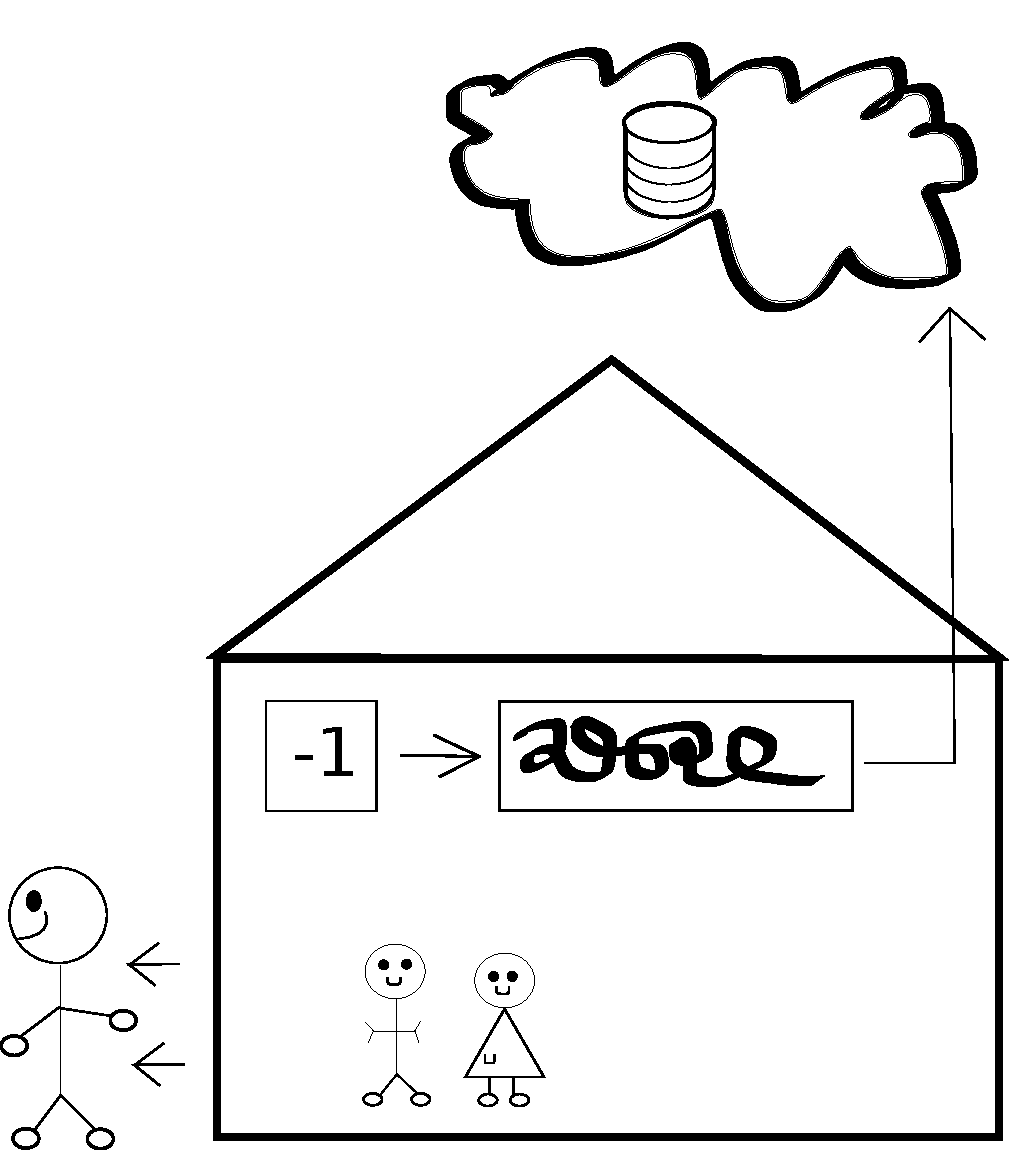
\includegraphics[width=0.65\linewidth]{casestudy}}\\}

  }

  \headerbox{Methodology}{name=methodology,column=1, row=0}{
    \begin{flushleft}A client-server architecture was designed and implemented in C++ to address a solution for the presented case study. Homomorphic encryption is enabled by using HElib [INSERTAR CITA]. Relevant tasks were divided between client and server.
    \end{flushleft}
    \noindent{\centering\fcolorbox{black}{white}{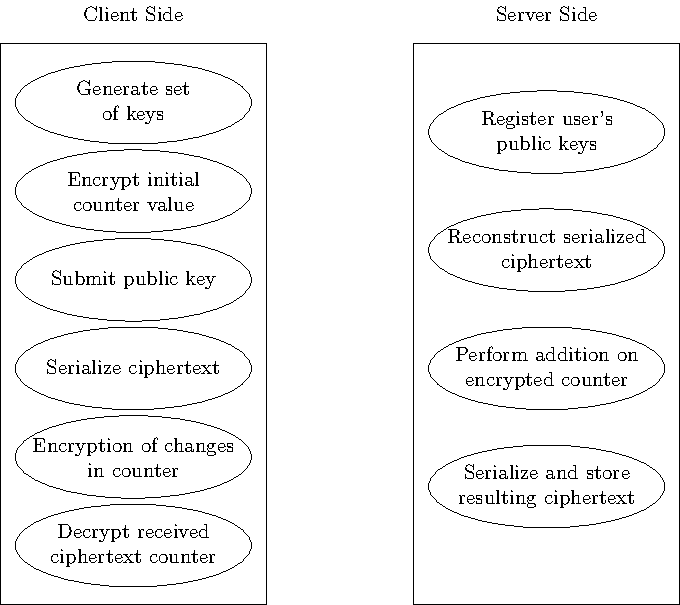
\includegraphics[width=0.65\linewidth]{architecture}}\\}
      
  }

  \headerbox{Operation Flow}{name=flow,column=1, below=methodology }{
    \noindent{\centering\fcolorbox{black}{white}{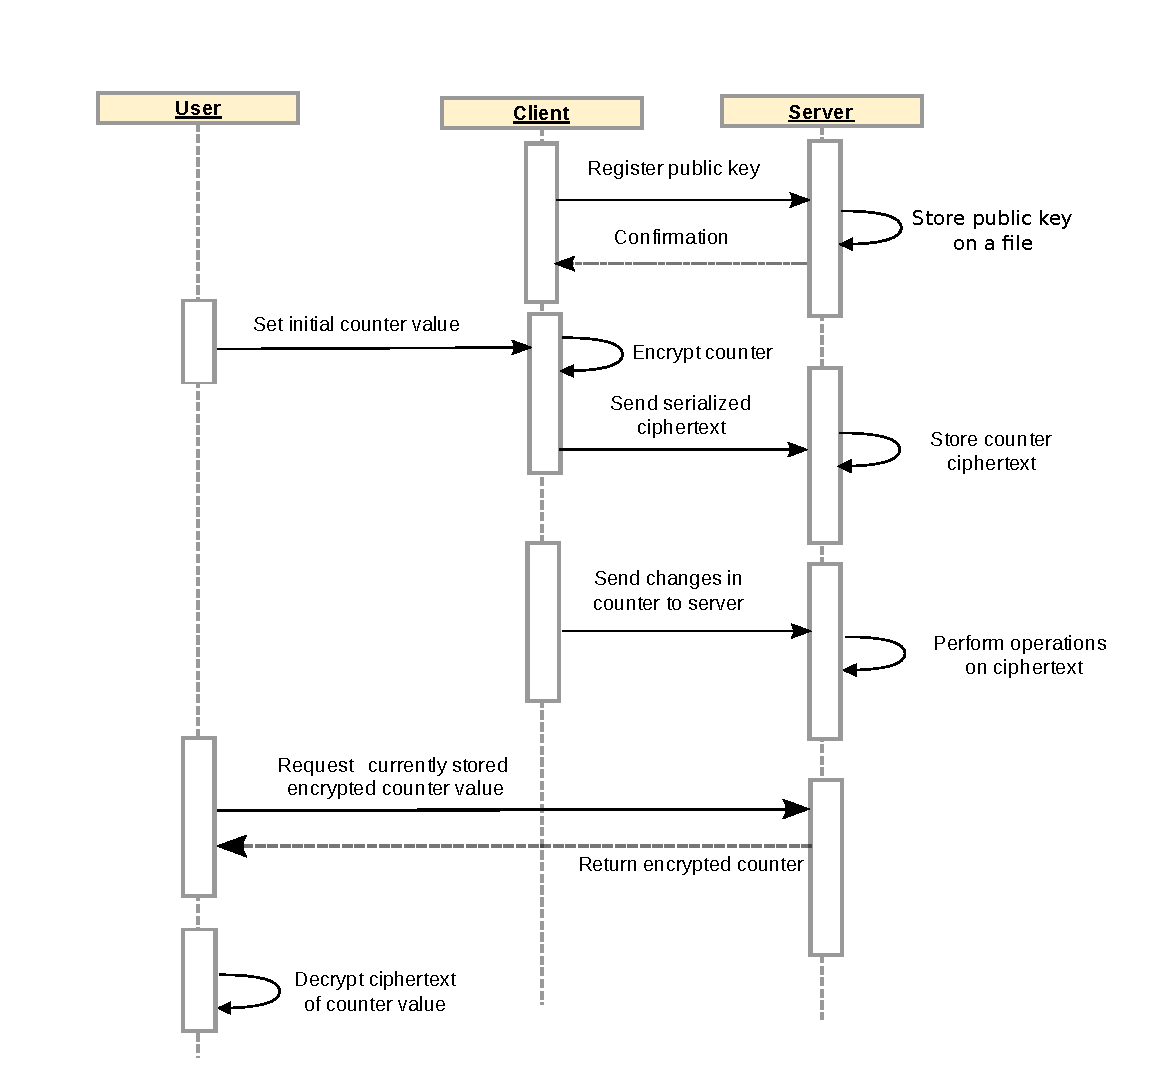
\includegraphics[width=0.95\linewidth]{counter}}\\}

  }
  
  \headerbox{Experimentation \& Results}{name=results,column=2,row=0}{
    \begin{flushleft}The performance of the system was evaluated by running 20 iterations with distinct values of a security parameter \emph{k} needed for the homomorphic encryption scheme. \\
      The system was evaluated in terms of ciphertext and key size, as well as the time needed for key generation and processing (addition, decryption, encryption).
    \end{flushleft}
    \noindent{\centering\fcolorbox{black}{white}{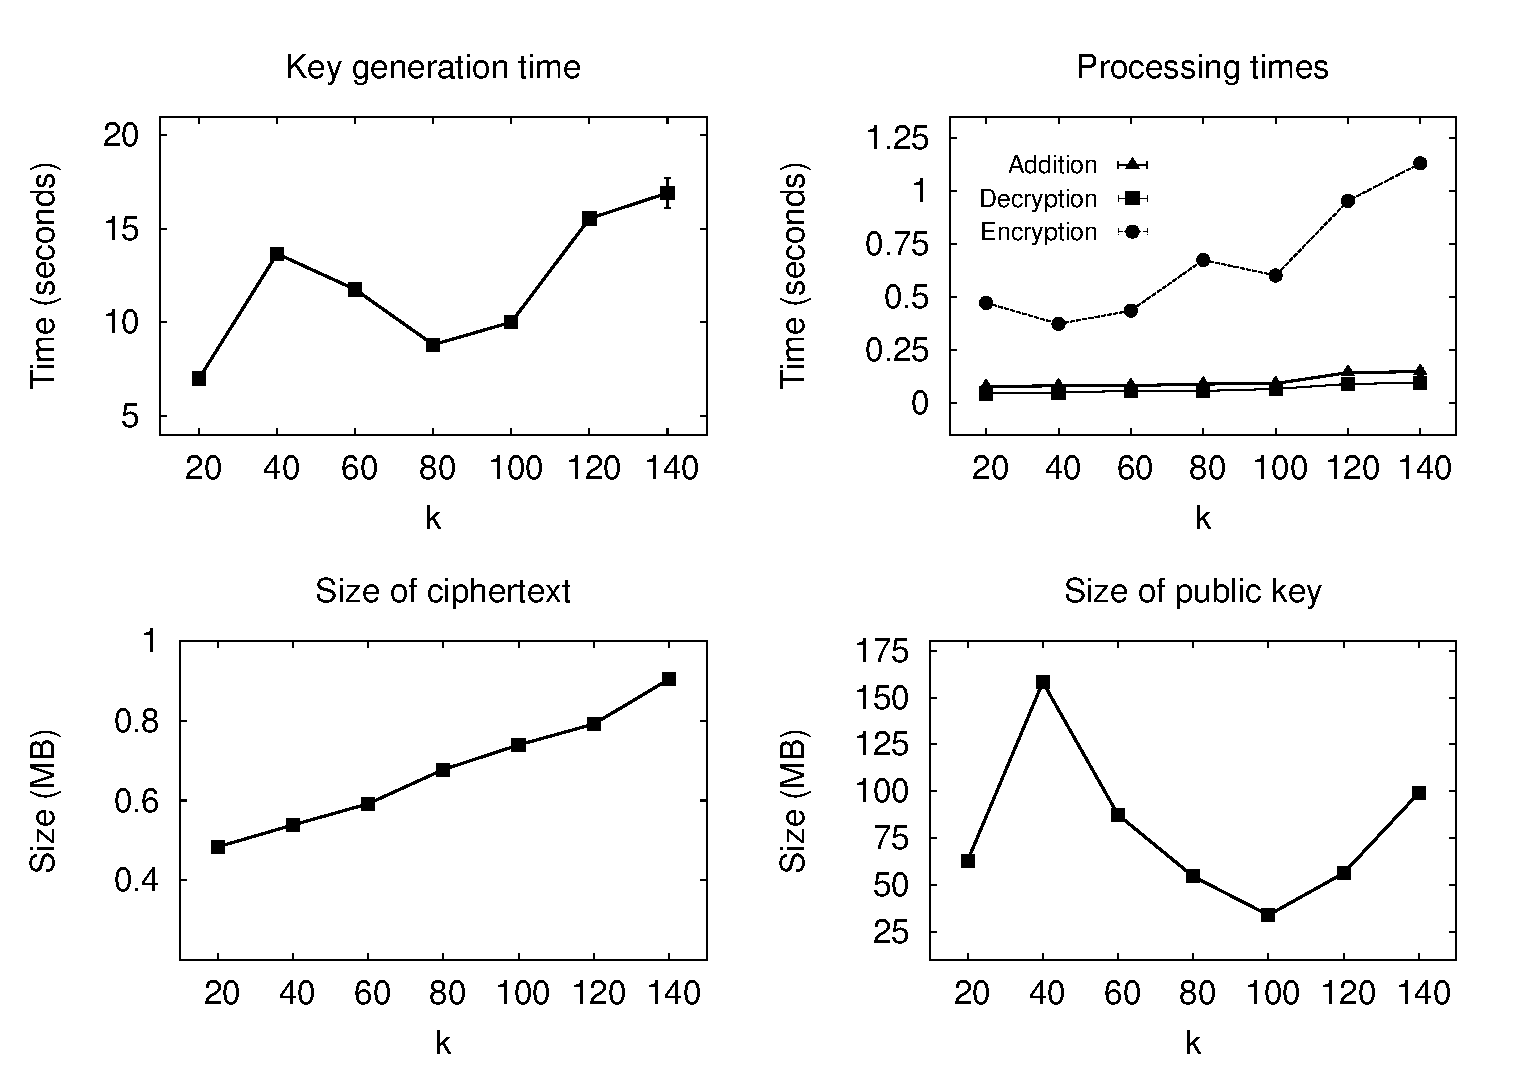
\includegraphics[width=0.95\linewidth]{proc}}\\}


  }

  \headerbox{Conclusions}{name=conclusions,column=2,below=results}{

  }

  \headerbox{References}{name=ref,column=2,below=conclusions}{    
    
  }


  \headerbox{Acknowledgements}{name=ack,column=2,below=ref}{    
    
  }

  \headerbox{Source Code}{name=code,column=2, below=ack}{
    https://github.com/antoniosv/homomorphic-counter  
  }
  
\end{poster}

\end{document}
